% !TEX TS-program = lualatex
%\documentclass[handout]{beamer}
\documentclass{beamer}
\input{../common/misomva}
\begin{document}
% Topic-specific title slide
\newcommand{\topictitle}{Natural Graphs Examples}
\newcommand{\topicsubtitle}{Biological, Information, and Utility Networks}
\newcommand{\misoclasstinytitleslide}{Partially based on material by:  Andreas Krause, \\[-1em] Branislav Kveton, Michael Kearns}

\MakeTopicSlide

\begin{frame}
\frametitle{Natural graphs from \emphcol{biological networks}}
\begin{columns}
\begin{column}{.5\textwidth}
\begin{itemize}\addtolength{\itemsep}{1\baselineskip}
\item protein-protein interactions  
\item gene regulatory networks
\item<+-> typical ML tasks 
\begin{itemize}\addtolength{\itemsep}{0.5\baselineskip}
\item discover unexplored interactions 
\item learn or reconstruct the structure
\end{itemize}
\end{itemize}
\end{column}
\begin{column}{.5\textwidth}
\begin{center}
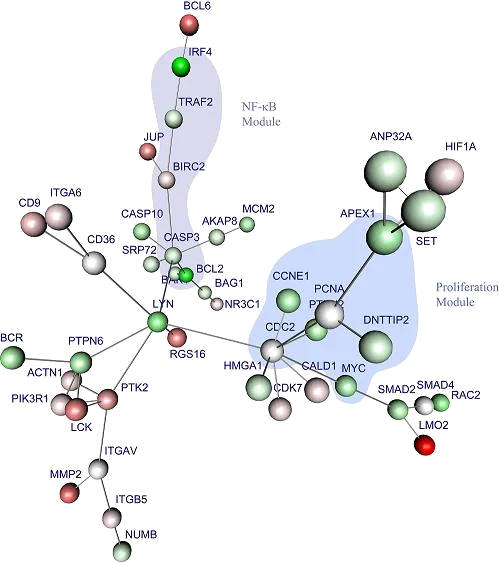
\includegraphics[width=\textwidth]{../img/bionetwork}\\
{\tiny Source: Basso et al. (2005)}
{\tiny Diffuse large B-cell lymphomas -  Dittrich et al. (2008)} 
\end{center}
\end{column}
\end{columns}
\end{frame}

\begin{frame}
\frametitle{Sources of Real Networks}
\begin{itemize}
\item \textbf{\url{https://ogb.stanford.edu/}}
\item \textbf{\url{http://snap.stanford.edu/data/}}
\item \url{http://www-personal.umich.edu/~mejn/netdata/}
\item \url{http://proj.ise.bgu.ac.il/sns/datasets.html}
\item \url{http://www.cise.ufl.edu/research/sparse/matrices/}
\item \url{http://vlado.fmf.uni-lj.si/pub/networks/data/default.htm}
\end{itemize}
\end{frame}

\begin{frame}
\frametitle{Constructed graphs from \emphcol{similarity networks}}
\begin{center}
\only<1|handout:1>{
\textbf{graph is not naturally given\\[1em]}%
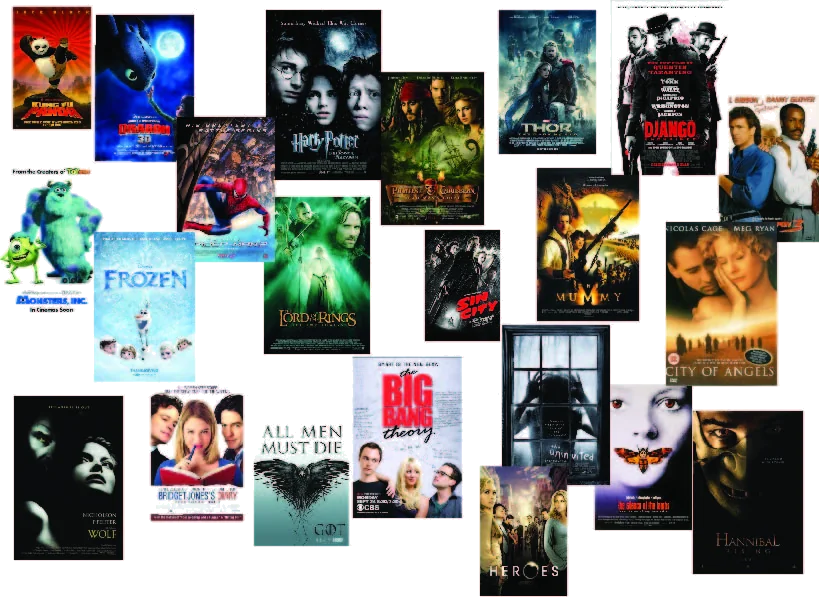
\includegraphics[width=0.8\columnwidth]{../img/movies1}}%
\only<2|handout:2>{
\textbf{but we can construct it\\[1em]}%
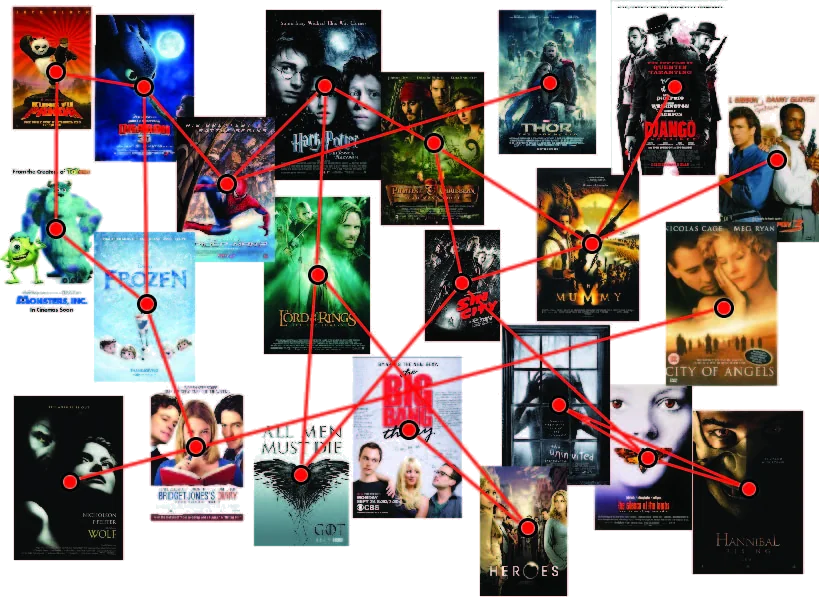
\includegraphics[width=0.8\columnwidth]{../img/movies2}}%
\only<3|handout:3>{
\textbf{and use it as an abstraction\\[1em]}%
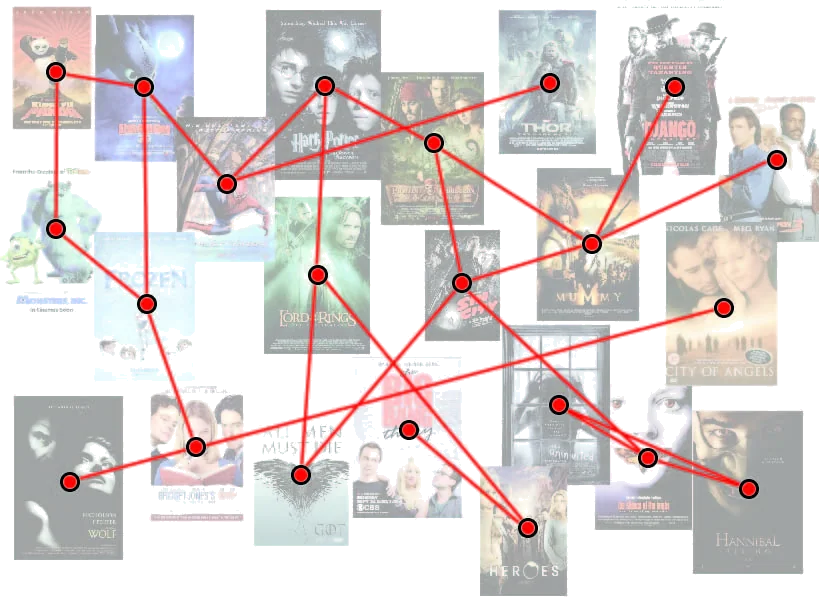
\includegraphics[width=0.8\columnwidth]{../img/movies3}}%
\end{center}
\end{frame}

\begin{frame}
\frametitle{Constructed graphs from \emphcol{similarity networks}}
\begin{columns}
\begin{column}{.5\textwidth}
\begin{itemize}\addtolength{\itemsep}{1\baselineskip}
\item vision  
\item audio
\item text  
\onslide<2|handout:1>{
\item typical ML tasks 
\begin{itemize}\addtolength{\itemsep}{0.55\baselineskip}
\item \textbf{semi-supervised learning  }
\item \textbf{spectral clustering}  
\item \textbf{manifold learning}
\end{itemize}
}
\end{itemize}
\end{column}
\begin{column}{.5\textwidth}
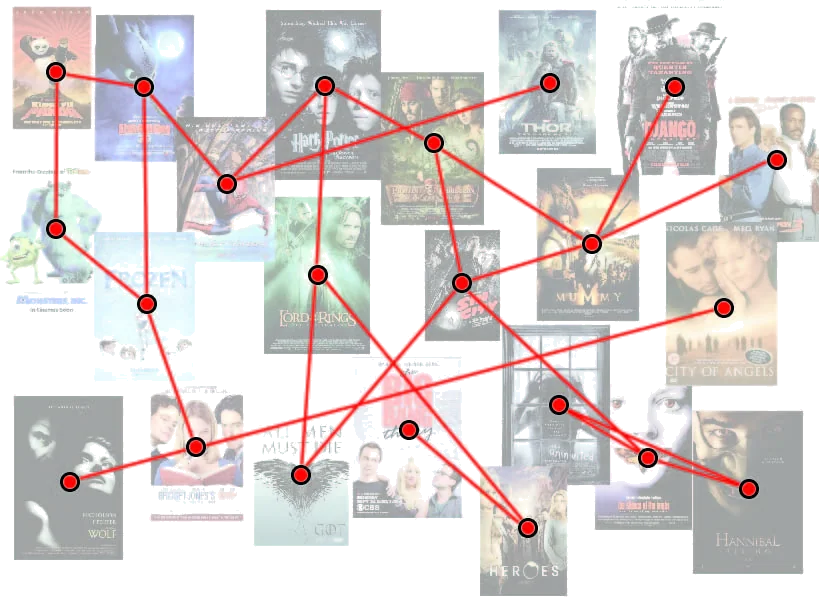
\includegraphics[width=\textwidth]{../img/movies3}\\
{\small movie similarity} 
\end{column}
\end{columns}
\end{frame}







\MakeLastSlide
\end{document}
